\documentclass[sigconf]{acmart}

\usepackage{graphicx}
\usepackage{algorithm} % for algorithms
\usepackage{algpseudocode}
\algblockdefx[Process]{Process}{EndProcess}[2][Unknown]{{\bf Process} {\it #2}}{}
\algblockdefx[Event]{Event}{EndEvent}[2][Unknown]{{\bf upon event #2 do}}{}

\usepackage{booktabs} % For formal tables
%\usepackage{cite} %for multiple refs

\usepackage{amssymb} %for nice emptyset

\usepackage{amsmath}
\DeclareMathOperator{\rank}{rank}
\makeatletter
\newenvironment{sqcases}{%
  \matrix@check\sqcases\env@sqcases
}{%
  \endarray\right.%
}
\def\env@sqcases{%
  \let\@ifnextchar\new@ifnextchar
  \left\lbrack
  \def\arraystretch{1.2}%
  \array{@{}l@{\quad}l@{}}%
}
\makeatother

\usepackage{amsthm}
 
\theoremstyle{definition}
\newtheorem{definition}{Definition}

\settopmatter{printacmref=false, printccs=true, printfolios=true}
\pagestyle{plain} % removes running headers

\newcommand{\PicScale}{0.5}
\newcommand {\FlameStream} {Icetream}
\begin{document}

\title {A formalization of consistency guarantees for distributed stream processing}

% \author{  Igor E. Kuralenok,$^1$     Artem Trofimov,$^ {1,2}$    Nikita Marshalkin,$^ {1,2}$   and  Boris Novikov$^ {1,2}$ }
% \affiliation{%
% \institution{$^1$JetBrains Research}
%   \city{St. Petersburg} 
%   \country{Russia}
% }
% \affiliation{%
% \institution{$^2$Saint Petersburg State University}
%   \city{St. Petersburg} 
%   \country{Russia}
% }
% \email{\string{ikuralenok, trofimov9artem, marnikitta\string}@gmail.com, borisnov@acm.org}

% \begin{abstract}
% Currently, large-scale distributed stream processing is a hot area of research. While state-of-the-art distributed stream processing systems are able to provide low-latency under at-most-once and at-least-once guarantees, achieving exactly-once semantics is still a challenging problem. An important reason behind this fact was the lack of efficient implementation techniques for idempotent stream processing model. In this work, we apply a low-overhead deterministic model to the problem of exactly-once. We demonstrate the lightweight protocols which use the property of determinism for achieving system-wide idempotence, and, therefore, exactly-once. Our experiments show that proposed approach can significantly outperform an alternative industrial solution.
% \end{abstract}

\maketitle

\section{Preliminaries}

In this section, we remind main concepts of stream processing, which we use further in this paper. Basically, a distributed stream processing system is a shared-nothing distributed runtime, that can handle a potentially unlimited sequence of input items. Each item can be transformed multiple times before the final result is released from the system. Elements can be processed one-by-one or grouped into small input sets, usually called {\em micro-batches}. 

An element has been {\em entered} if the system is aware of this element since that moment and takes some kind of responsibility for its processing. This concept can be implemented in a different way in different systems. For example, in Flink the fact that the element has been entered means that the element has arrived at {\em Source} vertex. In Spark Streaming, element enters, when it is read or received by an input agent also called {\em Source}. 

An element has {\em left} the system if an element has been released to a consumer. Since that time system cannot observe it anymore. This concept can also be implemented differently in various systems. For instance, in Spark Streaming element leaves when it is pushed to output operation, .e.g., written to HDFS or file. In Flink element leaves when it leaves from {\em Sink} vertex.   

It is important to note that input and output elements cannot be directly matched due to a possibility of complex transformations within the system. For instance, a single input element can be transformed into multiple ones. Hence, in a general case, it is impossible to determine input element by an output.

The way how a system transforms input elements is usually defined in the form of a {\em logical graph}. A logical graph is a graph, typically set up by a user, where vertices are {\em business-logic} operations and edges determine the order of processing. Each user-defined operation may be {\em stateless} or {\em stateful}. States of operations are usually managed by the system itself to prevent inconsistencies.

The main difference between the state of user-defined operation and an ordinary element is that the state is consumed, updated, and produced by the same operation. In~\cite{we2018adbis} it is shown that operations state can practically be an ordinary data flow element for any stateful operation. Therefore, without loss of generality, we can assume that the states of operations are just special elements in a data flow.

\section {Motivation}

In state-of-the-art stream processing systems~\cite{carbone2015apache, apache:storm, Zaharia:2016:ASU:3013530.2934664} a contract with end-user regarding ~{\em which data} will be eventually processed and released in case of failures is usually described in terms of so-called~{\em delivery guarantees}. These guarantees include {\em at most once}, {\em at least once}, and {\em exactly once}. {\it At most once} states that each input event is processed once or not processed at all. {\it At least once} guarantees that each input item is processed, but possibly multiple times, that can lead to result duplication. {\it Exactly once} assures that each input event is processed exactly one time.

A tricky thing in these seemingly simple definitions is that output item depends not only on the corresponding input item but also on the {\em state} of data flow operations and on the other elements in a data flow. This fact implies that a system can {\em technically} support exactly once delivery guarantee, but in practice can release completely invalid results, because of inconsistencies in the state or in-flight elements. Another vague point is the possibility of the generation of multiple elements from one inside a data flow. If these elements are applied to state or released non-atomically, it can lead to inconsistencies as well. State-of-the-art stream processing systems avoid these types of inconsistencies using complex recovery and state management mechanisms~\cite{Carbone:2017:SMA:3137765.3137777}. In terms of these systems, exactly once or at most once is not only about delivery but is also about {\em consistency}. We believe that such meaning is much more reasonable, and further in this paper, we will call them {\em consistency guarantees}.   

However, lack of formalism in the definitions of such streaming consistency guarantees is constantly causing debates and misunderstandings~\cite{JerryPengStreamIO, PaperTrail}. There is a need to introduce formal definitions in order to describe what exactly state-of-the-art stream processing engines guarantee. Such formalisms can also help to illustrate the differences between existing approaches.

In order to make our mathematical model independent of any implementation, we consider streaming consistency guarantees as correspondences between input and output streams and system state. If we formulate guarantees only in these terms, they can be applied to any system. However, the question of what to consider as a system state is a little bit sophisticated. At a very high-level, we can define a state as a {\em information} about input elements, which have been previously entered the system.  

An obvious idea is to say that system state is a state of user-defined operations, i.e., so-called {\em business logic} state. The main purpose of the states of operations is to accumulate the information about input items. It allows a system to not store all previous input elements in order to process a new one in a stateful user-defined operation. However, output items can be affected not only by input ones and operations state but also by other elements, which are currently in the system. For instance, if cycles are allowed in a logical graph, cycling elements can affect output ones, but they do not belong to a state. In-flight elements can also influence the result, being not in the state. These examples demonstrate the evident fact that information about input elements can be contained not only in the states of operations but in data flow elements as well.

\section{Formalization of consistency guarantees}

Facing the facts discussed above, let us try to dive into the internals of stream processing. Let $\tau\in{\mathbb{N}}$ be an exact global discrete time. Let $a_\tau$ be the element, which enters at the time $\tau$, and $b_\tau$ is the element, which leaves at the time $\tau$. 

\begin{definition}{System state}
$W_\tau$ at the time $\tau$ is the set of elements, which are currently in the system, $W_0=\emptyset$. There are only three ways to modify this set:

$W_{\tau+1}=\begin{sqcases}
W_{\tau}\cup{a_\tau}, & \text{or}\\
W_{\tau}\setminus{b_{\tau+1}}, & \text{or}\\
W_{\tau}\setminus{X}\cup{Y}, X\subseteq{W_\tau},{Y}\subseteq{W_{\tau+1}} & \text{}.
\end{sqcases}$

\end{definition}

The last expression illustrates elements transformation. There are two possible scenarios. The first one is a transformation into other elements due to, e.g., map operation. The second case is combining elements and states of operations into the new states. As it was mentioned above, states of operations can be considered as ordinary elements in the system without loss of generality. Hence, $W_\tau$ is a valid system state, because it contains both operations state and all elements, which are currently in the system, i.e., it contains a complete information about the elements, which have been already entered.

\begin{definition}{Operations state or business-logic state}
$S_\tau$ at the time $\tau$ is $W_\infty$ if $\forall t>\tau: a_t=\emptyset$.
\end{definition}

% In this setting, we can define operations state $S_\tau$ as $W$ if there are no input elements since time $\tau$, i.e. $\forall t>\tau: a_t=\emptyset$. Let us denote it as $S_\tau=W^{\infty}_\tau$. 

We can imagine a stream processing system as a pool, where some elements are poured in and others are poured out. The business logic states are the elements, which are kept in the pool if we stop pouring in and wait infinite time.

\begin{definition}{Dependency relation}
$D$ is a transitive binary relation $D\subseteq{{\bigcup^{\infty}_{i=1}{W_i}}\times{{\bigcup^{\infty}_{i=1}{W_i}}}}$. Pair $(x,y)\in{D}$ iff $\exists{\tau,X,Y}:W_{\tau+1}=W_\tau\setminus{X}\cup{Y}, x\in{X}, y\in{Y}$.
\end{definition}

Here we can draw an analogy with {\em Herbrand semantics}, where the notion of dependency is used to describe on which transactions, current write operation depends on. Write operation depends on a transaction if the transaction is active. Therefore, commit is a defined point, since then a transaction cannot affect further writes. In our model, there is also a need to define such moment, since then there are no elements in a system, which depend on $a_\tau$, except the business-logic state.

\begin{definition}{Nullification time}
of an input element $a_\tau$ is the time $\theta_{a_\tau}=inf(\hat{\tau}>\tau|W_{\hat{\tau}}\setminus{S_{\hat{\tau}}}\cap{Cl(D)(a_\tau)=\emptyset})$, where $Cl(D)$ is a transitive closure of the relation $D$.
\end{definition}

Nullification time is a key concept within our model. It allows us to observe a moment when an input element starts to affect output elements only through the state. It should be noted that nullification is not only a theoretical concept, because it can be practically observed using, e.g., low watermarks or punctuations~\cite{Tucker:2003:EPS:776752.776780}. The concept of nullification is shown in Figure~\ref{nullification}.

\begin{figure}[htbp]
  \centering
  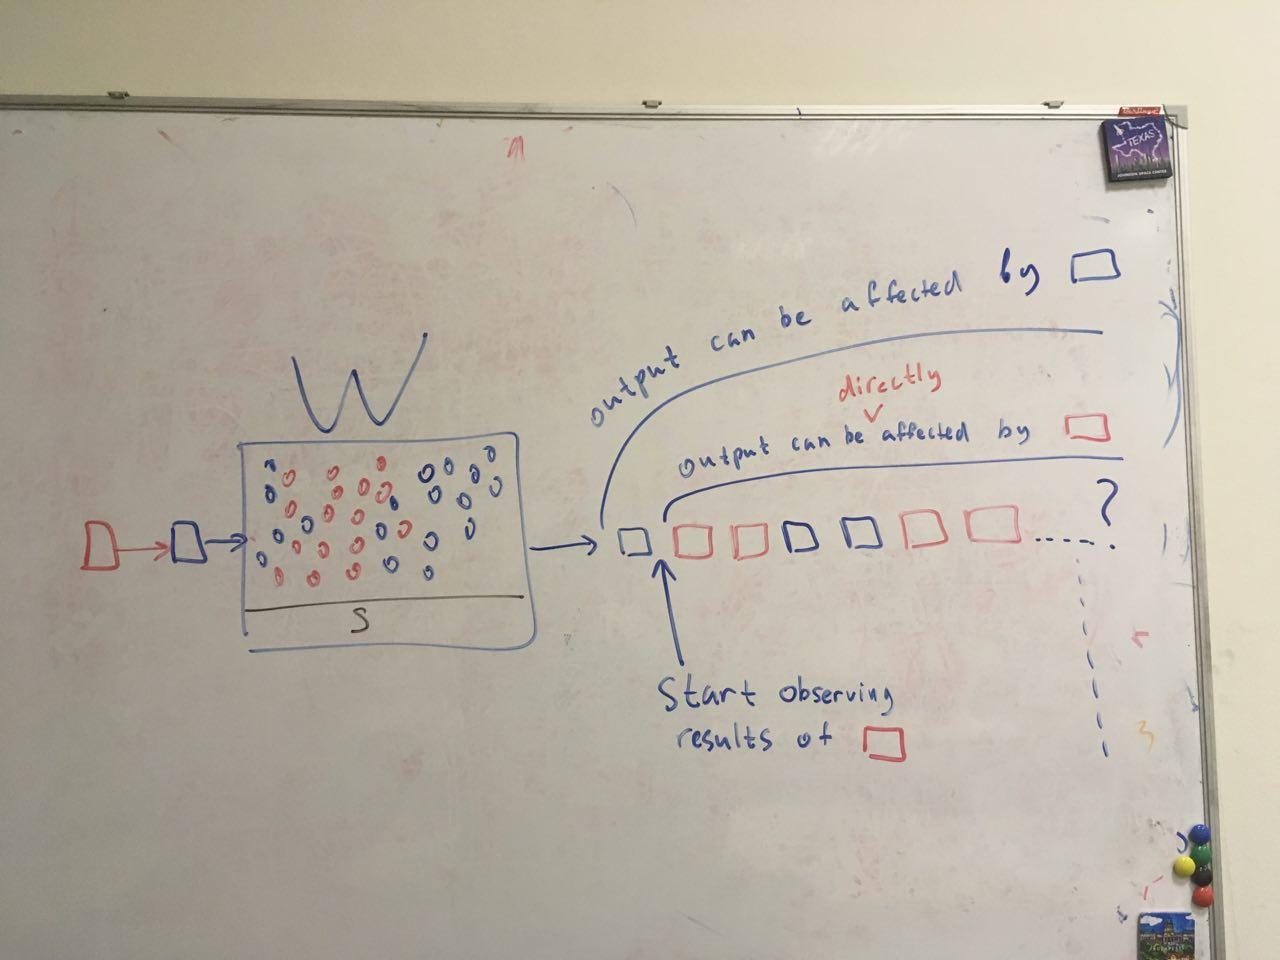
\includegraphics[width=0.48\textwidth]{pics/nullification}
  \caption{The red and blue elements have entered the system. Since that time, it is unclear, when they stop directly affect output elements}
  \label {nullification}
\end{figure}

\begin{definition}{Time quantization}
$t$ is the times of input, output, and nullification:

$t=\begin{cases}
\tau_i:\exists{a_{\tau_i}}, \\
\tau_o:\exists{b_{\tau_o}}, \\
\theta_{a_\tau}.
\end{cases}$
\end{definition}

The main purpose of time quantization is to provide observable points in time. Further, we will consider a system only in terms of time $t$. Now we can model a system state and output elements for the cases of different input sets at some defined points in time. 

Let $x,a_1,a_\infty$ be input elements with arbitrary arrival times. $\mathbb{B}_t$ is all output elements by the time $t$:

$\mathbb{B}_t=\bigcup\limits_{i=1}^{t}{b_i}$

Let $p(W_t,\mathbb{B}_t|x,a_1...a_\infty)$ be a probability to observe state $W_t$ and output elements $B_t$ at the time $t$ if input elements are $x,a_1,a_\infty$. Let us construct three sets:

$X^0=(W_\infty,\mathbb{B}_\infty|p(W_\infty,Q_\infty|a_1...a_\infty)\neq{0})$

$X^1=(W_{\theta_{x}},\mathbb{B}_{\theta_{x}}|p(W_{\theta_{x}},Q_{\theta_{x}}|x,a_1...a_\infty)\neq{0},\forall{i}:{a_i}\neq{x})$

$X^{*}=(W_{\theta_{x}},\mathbb{B}_{\theta_{x}}|p(W_{\theta_{x}},Q_{\theta_{x}}|x,a_1...a_\infty)\neq{0},\\
\exists{i}:{a_i={x}},\exists{y:y\in{W_{\theta_{x}}\setminus{S_{\theta_x}}}\cap{Cl(D)(a_i)}})$

These sets model the {\em observable} output and state of a stream processing engine. $X^0$ expresses the case, when element $x$ has not affected the system state and the output, so it is a forbidden behavior for at least once and exactly once guarantees. On the other hand, $X^{*}$ defines possible results, after $x$ has been nullified, but $a_i=x$ or its dependencies are in the system. Such behavior can cause inconsistencies in operations state due to duplicates and should not be observed if the system provides for at most once or exactly-once. Using these modeled sets now we can define guarantees.

\begin{definition}{At most once}
guarantee is provided by a system iff $\forall{x,a_1...a_\infty}:X^{1}\cap{X^{*}}=\emptyset$
\end{definition}

\begin{definition}{At least once}
guarantee is provided by a system iff $\forall{x,a_1...a_\infty}:X^{0}\cap{X^{1}}=\emptyset$
\end{definition}

\begin{definition}{Exactly once}
guarantee is provided by a system iff $\forall{x,a_1...a_\infty}:X^{0}\cap{X^{1}}\cap{X^{*}}=\emptyset$
\end{definition}

Now streaming consistency guarantees are defined in terms of correspondences between input, output and the system state. Custom system or user-defined semantics are not considered in this model, e.g., if the system drops all input items, it also can be claimed as supporting exactly-once. Looking from another side, our model formally describes which properties are {\em exactly} supported by state-of-the-art stream processing systems, such as Flink, Storm, Spark Streaming, Samza, etc, so we can discuss its properties in unified terms. What is more important, we demonstrated that guarantees, which are misleadingly called {\em delivery}, in practice affect data {\em consistency} as well.









% Facing this fact, we can consider the system state as operations state together with all elements, which are currently in the system. Let $\tau$ be an exact global discrete time. Let $a_\tau$ be the element, which enters at the time $\tau$, and $b_\tau$ is the element, which leaves at the time $\tau$. Let $W_\tau$ is the set of elements, which are currently in the system, $a_\tau\in{W_\tau}$, $b_\tau\notin{W_\tau},b_\tau\in{W_{\tau-1}}$. As it was mentioned above, we assume that the states of operations are elements in the system as well, so if $S_\tau$ is the set of states of operations at time $\tau$, then $S_\tau\subseteq{W_\tau}$. We can define $S_\tau$ as $W_\infty$ if there are no input elements since time $\tau$, i.e. $\forall t>\tau: a_t=\emptyset$. Let us denote it as $S_\tau=W^{\infty}_\tau$. We can imagine stream processing system as a pool, where some elements are poured in and others are poured out. The states are the elements, which are kept in the pool if we stop pouring in and wait infinite time.

% Let us consider $W_\tau$ as a system state, i.e., the system state is operations state together with all elements, which are in the system at the time $\tau$. At the time $\tau+1$, $W_\tau$ can be changed by one of the following atomic events:

% \begin{enumerate}
%     \item Element enters the system
%     \item Element leaves the system
%     \item Element is transformed into an operation state and/or other elements
% \end{enumerate}

% More formally,

% $W_{\tau+1}=\begin{cases}
% W_{\tau}\cup{a_\tau}, & \text{or}\\
% W_{\tau}\setminus{b_{\tau+1}}, & \text{or}\\
% W_{\tau}\setminus{x}\cup{\{y_i\}}, & \text{}.
% \end{cases}$

% It can be said that an element depends on other one, if it is a result of transformation. Let us denote this as a transitive binary relation $D$. Let $Cl(D)$ be a transitive closure of $D$. 














% In order to make our mathematical model independent of any implementation, we consider streaming consistency guarantees as correspondences between input and output streams and the state. If we formulate guarantees only in these terms, they can be applied to any system. As it was mentioned above, each input element can be transformed into multiple ones and so on. Hence, in a general case it is not possible to determine input element by output one. Because of this fact, it is unclear at which point in time an element is {\em nullified}, i.e. system does not contain the element itself and elements generated from it.  













% {\em State machine} is a natural and convenient way to express such correspondences~\cite{ссыль}. We can consider the whole stream processing system as a state machine. In this case, the state is a state of dataflow operations together with a set of items, which are being processed in the system at the moment. The events in such state machine are not only arrivals of input elements, but also such moments when input elements have been {\em nullified}. It means that the element has been completely processed or lost. However, it is unclear how to define such moments in a general case. Let us introduce some concepts, which allow us to do it.

% Three basic concepts can be different for different stream processing engines. However, generality is not lost, because the specific implementation does not influence the model. The first concept is {\em entering} to the system. For example, in Flink the fact that the element has been entered means that the element has arrived at {\em source} vertex. The second notion is {\em leaving} from the system. For example, it means that element has been released to a consumer or lost. The third one is a {\em dependency}. We say that element $b$ depends on the element $a$ if $a$ has been involved in the creation of $b$. In practice, it means, e.g., that $b$ has been generated from $a$ using flat map operation. It is assumed that the states of dataflow operations are just data elements in the system, which are independent of any other elements.

% Using these basic definitions, we can introduce the remaining necessary ones. Let $\tau$ be a global discrete time. Let $W_\tau$ is the set of {\em working} elements at the time $\tau$. Working elements at the time $\tau$ are the elements which have already entered the system or generated inside the system at the time $\geqslant{\tau}$, but have not left it yet. Because of the assumption that states of dataflow operations are just independent elements in the system, they are also contained in the set of working elements, i.e. if $S$ is the set of operation states, then $S\subseteq{W_\infty}$. Let $x_\tau\in{W_\tau}$ be the element, which enters at the time $\tau$, and $q_\tau\notin{W_\tau},q_\tau\in{W_{\tau-1}}$ is the element, which leaves at the time $\tau$. Let $D_{x_{\tau}}$ be the set of elements, which depend on $x_\tau$.

% Having the definitions introduced above, now we can define the meaning of an element nullification. We say that element $x_\tau$ is nullified at time $\eta_{x_{\tau}}$ if $\eta_{x_{\tau}}$ is the minimal time, when $\nexists{y\in{W_{\eta_{x_{\tau}}}}}:{y}\to{x_{\tau}}$, where $\to$ is a transitive dependency. More formally, $\eta_{x_{\tau}} = inf(\hat{\tau}:\hat{\tau}\geqslant{\tau}\land{\nexists{y\in{W_{\eta_{x_{\hat{\tau}}}}}}:{y}\to{x_{\hat{\tau}}}})$. Therefore, in the proposed model events occur when an element is arrived and nullified, i.e., at times $t_i:\exists{x_{t_i}}$ and $t_o:\exists{\eta_{x_{t_o}}}$. In other words, we define time quantization for the state machine.

% Now we can compare the sets of working and left elements for the cases of different input sets at some defined points in time. The main idea here is to express at most once, at least once, and exactly once guarantees as interactions between such sets. Let $x,a_1,a_\infty$ be input elements with arbitrary arrival times. $Q_\tau$ is all output elements by the time $\tau$:

% $Q_\tau=\bigcup\limits_{i=1}^{\tau}{q_i}$

% Let $p(W_\tau,Q_\tau|x,a_1...a_\infty)$ be a probability to observe state $W_\tau$ and output elements $Q_\tau$ at the time $\tau$ if input elements are $x,a_1,a_\infty$. Let us construct three sets:

% $X^0=(W_\infty,Q_\infty|p(W_\infty,Q_\infty|a_1...a_\infty)\neq{0})$

% $X^1=(W_{\eta_{x}},Q_{\eta_{x}}|p(W_{\eta_{x}},Q_{\eta_{x}}|x,a_1...a_\infty)\neq{0},\forall{i}:{a_i}\neq{x})$

% $X^{*}=(W_{\eta_{x}},Q_{\eta_{x}}|p(W_{\eta_{x}},Q_{\eta_{x}}|x,a_1...a_\infty)\neq{0},\exists{i}:{a_i={x}},\exists{y\in{W_{\eta_{x}}}}:y\to{a_i})$

% These sets model the {\em observable} output and state of a stream processing engine. $X^0$ expresses the case, when element $x$ has not affected the state and the output, so it is a forbidden behavior for at least once and exactly once guarantees. On the other hand, $X^{*}$ defines possible results, after $x$ has been nullified, but $a_i=x$ or its dependencies are in the system. Such behavior can cause inconsistencies in operations state due to duplicates and should not be observed if the system provides for at most once or exactly-once. We define consistency guarantees as follows: 

% {\em At most once} $\iff$ $\forall{x,a_1...a_\infty}:X^{1}\cap{X^{*}}=\emptyset$

% {\em At least once} $\iff$ $\forall{x,a_1...a_\infty}:X^{0}\cap{X^{1}}=\emptyset$

% {\em Exactly once} $\iff$ $\forall{x,a_1...a_\infty}:X^{0}\cap{X^{1}}\cap{X^{*}}=\emptyset$

% Now streaming consistency guarantees are defined in terms of correspondences between input, output and the state. Custom system or user-defined semantics are not considered in this model, e.g., if the system drops all input items, it also can be claimed as supporting exactly-once. Looking from another side, our model formally describes which properties are {\em exactly} supported by state-of-the-art stream processing systems, such as Flink, Storm, Spark Streaming, Samza, etc, so we can discuss its properties in unified terms. What is more important, we demonstrated that guarantees, which are misleadingly called {\em delivery}, in practice affect data {\em consistency} as well.

\subsection{Additional properties and notes}
 
 TBA

\bibliographystyle{ACM-Reference-Format}
\bibliography{../../bibliography/flame-stream.bib}
\end {document}

\endinput
you can put whatever here
